\chapter{Results}\label{chap:results}


%Describe the experimental setup, the used datasets/parameters and the experimental results achieved

This section gives an overview of the used datasets, the used metric to evaluate our models, the configuration of our model and finally, the experimental results achieved.

\section{Dataset}\label{sec:dataset}
In this implementation we only used the text8 \footnote{http://mattmahoney.net/dc/enwik8.zip} dataset. We chose this dataset for two reasons. First of all, its a very small dataset, that allowed us to do a lot of computations. Secondly, this data set was used in a lot of related work \cite{gpu}, \cite{cpu} hence giving us a very good benchmark. The text8 dataset consists of 1702 lines of 1000 words, with a vocabulary of roughly 63000 words. Conventienly, there is no punctuation in the dataset. Therefore, we had to choose between building arbitrary sentences and keeping the dataset as it is. We chose the first option because it gives us a faster computation time, and did not show any significant loss in quality empirically, as shown in Table \ref{table:with_20}. We chose a length of sentences of 20. Furthermore, we applied a technique called subsampling to reduce the data set size, which is explained in the following section. 

\begin{table}[]
\centering
\begin{tabular}{|l|l|l|l|l|}
\hline
Length of Sentences        &  10  & 20   & 40    & 1 Document \\ \hline
Training Time for one batch  &8min & 10min  &  11min  & 18min      \\ \hline
Convergence Time &4 epochs & 3 epochs & 3 epochs & 3 epochs   \\ \hline
Word Similarity& 0.65  & 0.66 & 0.66    & 0.66       \\ \hline
\end{tabular}
\caption{Training and Convergence time according to choice of the length of sentences in text8 dataset}
    \label{table:with_20}
\end{table}


 
\subsection{Subsampling}
Subsampling is a technique introduced by Mikolov et al. \cite{mikolov} to reduce the dataset size while at the same time increasing the quality of the dataset, i.e getting better word embeddings with it. The idea behind subsampling is the removal of very frequent words such as: "the, as, it, of". These words do not give an intrinsic value to the words that appear in its context. Therefore the goal of subsampling is to delete such words from the dataset. This will decrease the computation time, as it will reduce the number of training samples, and should, in theory, increase the accuracy of the model. The increase in accuracy can also be explained by the fact that words that would not have appeared in the context of each other, may know do because words between have been deleted.
To choose which word to delete,  Mikolov et al. \cite{mikolov2} chose the following equation to compute the deletion of a word $w$ in the data set:
\begin{equation} \label{eq:sampling}
P(w) = 1- \sqrt{{\frac{t}{f(w)}}}
\end{equation}

where $f(w)$ is the frequency of w, and $t$ is a threshold set empirically. As Equation \ref{eq:sampling} is a probability, subsampling is not a deterministic procedure, words that may have been deleted with a threshold of $10^-2$ may stay in the dataset with a lower threshold, as shown in Table \ref{table:treshold_examples}. Mikolov et al. recommend a value between $0$ and $10^{-5}$, depending on the size of the dataset. We experimented with different values and $10^{-4}$ seemed the most suited. We did this by looking at a random set of sentences and judging the results manually. An example of the first sentence with different sampling thresholds can be found in Table \ref{table:treshold_examples}. The table shows the first 20 words of our dataset, without the words that were subsampled according to a threshold sample. Stats about subsampling can be found in Table \ref{table:treshold}. 
\begin{table}[h]
\centering
\begin{tabular}{|l|l|l|l|l|l|}
\hline
Sampling Treshhold &  0      &      $ 10^{-1}$&$   10^{-2}$& $10^{-3}     $ &$10^{-4}   $    \\ \hline
Number of words in Dataset    & 16 mio & 15mio & 11 mio & 8mio & 4 mio \\ \hline
\end{tabular}
\caption{Size of the preprocessed text8 dataset according to sampling treshold}
\label{table:treshold}
\end{table}

\begin{table}[]
\begin{tabular}{|l|l|}
\hline
Sampling Treshold & First sentence of Dataset                                                                                                                                               \\ \hline
$10^{-1}$           & \begin{tabular}[c]{@{}l@{}}Anarchism originated as a term of abuse first used against early\\  working class radicals including the diggers of the english\end{tabular} \\ \hline
$10^{-2}$           & \begin{tabular}[c]{@{}l@{}}Anarchism originated as a term of abuse first used against early \\ working class radicals including diggers of english\end{tabular}         \\ \hline
$10^{-3}$           & \begin{tabular}[c]{@{}l@{}}Anarchism originated  a term  abuse first used against early \\ working class radicals including  diggers the english\end{tabular}           \\ \hline
$10^{-4}$           & \begin{tabular}[c]{@{}l@{}}Anarchism originated abuse used against working class radicals\\ diggers english\end{tabular}                                                \\ \hline
$10^{-5}$           & against radicals diggers                                                                                                                                                \\ \hline
\end{tabular}
    \caption{Example of a sentence with different sampling tresholds}\label{table:treshold_examples}
\end{table}
\subsubsection{Min count}
We also deleted every word that did not appear more than 5 times in our dataset. We got this technique from Gensim \cite{gensim}, that introduced this parameter into their training. This is a good technique because of three reasons: First certain words of our data sets do not appear in a common lexicon (twigleg, melqu), or come from a foreign language (Volksvereinigung), or are names and acronyms. Secondly, each document often has spelling mistakes, those (as long as the same spelling mistake does not appear too often, what should be avoided in practice) would be deleted by sampling too, as the words do not have any meaning. Lastly, a word that only appears one time in our dataset will be very dependent on its original initialization. This is the case because it will only be updated with its context pairs once, which is only a dozen of times in practice and then won't be updated any more. For all of the above reasons, we applied this technique. Similar to subsampling, it should in theory improve the quality of the word embeddings and will decrease the computation time. 

\section{Evaluating word embedings}
Evaluating word embedding is not an easy task, such as evaluating the accuracy of a common classifier. We cannot split our data set into train and test set. As the task that the network is learning is of no interest to us. Therefore we need to verify that our embedding is of quality with other techniques. To define quality we first need to define a measure of similarity between two vectors. This requires knowledge of the Cosine distance, which is introduced in the following section.
\subsection{Cosine distance}
The cosine similarity, this is not the cosine distance, of vectors $v$ and $w$ is the cosine of the angle between the two vectors It can be calculated by taking the dot product of $v$ and $w$ and dividing it by the magnitude of $v$ and $w$ multiplied with each other. We get:
\begin{equation}
cos\_sim(v,w) = \frac{v \cdot w}{|v| |w|} 
\end{equation}
The cosine of 0\textdegree ~is 1,  it's 0 for two vectors that are orthogonal to each other and vectors that point in the opposite direction will have a cosine of their angle of -1. This is not a good distance measure as -1 is smaller than 0, and therefore two vectors pointing away from each other would be closer than two orthogonal vectors, but by subtracting 1 from the cosine of the angle we can create a good distance measure between the two vectors. This distance does not take into account any order of magnitude. Hence for our tasks, two vectors will be considered equal if they are of different magnitude but point in the same direction. 
Apart from measuring the quality of word embedding well, this technique has another advantage. By normalizing the vectors the calculation of the cosine angle becomes the dot product of the two vectors. Which can be computed very fast on modern GPU's. 
Knowing that we have a measure to compute the similarity of two vectors let us introduce a way to rate the quality of our embeddings.


\subsection{Word similarity and wordsim353}
To measure the quality of our word embedding we will need a dataset to compare our results too. We chose  wordsim353\footnote{http://www.cs.technion.ac.il/~gabr/resources/data/wordsim353/wordsim353.zip} for this task, as it's the most used in the related literature. The data set consists of 353 pairs of words rated by humans on their similarity. The similarity score is in the range of 1 and 10, with 10 being the best score. An example for two of such pairs can be found in Figure \ref{fig:ws353_ex}. We will rank our embeddings on the Pearson correlation coefficient between the cosine distance and the scores attributed by humans, as this is a common procedure.

\begin{table}[]
\centering
\begin{tabular}{|l|l|l|}
\hline
Word1 & Word2 & Score \\ \hline
\textquote{FBI} & \textquote{Investigation} & \textquote{8.31} \\ \hline
\textquote{Mars} & \textquote{scientist} & \textquote{5.63} \\ \hline
\end{tabular}
   \caption{Example of pairs and their rating in wordsim353}
    \label{fig:ws353_ex}
\end{table}


\section{Configuration of the network}
The skip gram model has a lot of possible parameters, that can be tuned. We experimented with different models and finally decided for one that we tried to optimize. This section will give a short overview of each parameter, where we will explain the process in which we chose the value of the given parameter. The explanation of the parameters will be structured as follows: 
\texttt{Parameter} - Description and tuning -  \textit{Value}
\begin{itemize}
\item \texttt{Negative Samples:} Here we have to find a trade-off between, setting the parameter too high which will result in increased accuracy but a longer computation time. For smaller data sets a higher number of negative samples is often needed. In their original paper Mikolov et al. \cite{mikolov2} recommend a value of 5-20. We tested a few values in the range of 5 to 15, as 10 yielded state of the art results we chose this value. - \textit{10}
\item \texttt{Context Window:} The bigger the window the more training examples the network will have, but if the window is too big the semantic meaning of the window will be erased. Mikolov et al. \cite{mikolov} proposed a setting between 2-10, as all our sentences are of size 20 we chose 5. - \textit{5}
\item\texttt{ Dimension of the embedding}: Here the choice is less obvious, as the dimension needs to be high enough to capture the meaning, but cannot be too high as this leads to a decrease in performance as shown by Yin and Shen \cite{dimension_size}. We, therefore, used Gensim to find the best embedding possible. - \textit{100}
\item \texttt{Batch size}: As described in section \ref{ssec:b_SGM}, there is a tradeoff to find between quality and training time. We first used a batch size of 5000, but then decide after non conclusive results (see \ref{ssec:bs_lf}) that 2000 would be better - \textit{2000}
\item \texttt{Alpha}: learning rate, this hyperparameter was tuned in every optimizer therefore only the range will be indicated - \textit{(1e-5,1)}
\end{itemize}

\iffalse
\begin{table}[h]
\centering
\begin{tabular}{|l|l|}
\hline
Embedding Size & Word Similarity on Gensim \\ \hline
50 & 0.65 \\ \hline
100 & 0.67 \\ \hline
200 & 0.65 \\ \hline
300 & 0.63 \\ \hline
\end{tabular}
\caption{Word similarity in relation to the size of the embedding}
\label{table:gensim_emb_size}
\end{table}
\fi 
\section{Input Shuffling}
We used input shuffling as a technique to optimize the skip gram model. We will first describe input shuffling in a general way and then explain why we suppose that input shuffling could work well on the skip gram model. \\
Let $X = {x_1...x_n}$ be our input data set. Input Shuffling describes the process of taking a random permutation of the dataset as input at each epoch. 
The idea behind this technique is to present our optimizer with different loss surfaces so that it's able to find the best optimum. Therefore it's easier for the neural network to escape a local minimum. As for example if a network had converged to a local minimum after one epoch it could not escape it as all the parameters are the same. But if we change the shape of the loss function, by input shuffling, then there would be a greater probability for the network to escape the local minimum.
\\
There are two reasons why we think that input shuffling is particularly well suited for the skip gram model. The first one has to do with the fact that when we read our words sequentially that words that only appear very early will not benefit from the context words being already updated from others. The second idea is that we used the special batch technique described in Section \ref{ssec:b_SGM}. When using this technique and not using shuffling we will always have words that appear next to each other in a batch and will, therefore, update the same words at the same time. We, therefore, lose some quality. But if we would use input shuffling instead, then the words in one batch would likely not be similar and therefore only taking the average of a small part of pairs with the same words will be less likely. 


\section{Convergence time} 
To optimize convergence time we have to define it first. Therefore we used the already available implementation of Gensim \cite{gensim}. Gensim is an open source software that proposes an implementation of the SGNS in Python. It is also written in cython, therefore it has a fast computation time, but can be used inside a python implementation. Together with the knowledge from Ji et al.\cite{intel} that a score of $0.66$ in the task of word similarity, with the text8 dataset, is the state of the art, we tested Gensim (more on this process in Chapter \ref{chap:discussion} and found out that it took 4 epochs to converge. Therefore we defined the following criteria for convergence: \\
$\rho - \rho_{prev} < 0.009 \vee \rho = 0.66$ \\
where $\rho$ is the Pearson coefficient on the wordsim353 task. 
We also stopped computation, if it took more then 20 epochs to converge. 

\section{Results by optimizer}
We ran multiple experiments for each optimizer. This section will only give an overview of the achieved results. Each section will give an explanation over the achieved result with a specific optimizer.

\subsection{SGD}
The first challenge for each optimizer was to find a correct learning rate. As SGD is the optimizer used in Gensim \cite{gensim} we first tried the same learning rate as Gensim \cite{gensim} and then performed a random search to find a better one. As expected a bell curve shape resulted, a learning rate that is too high leads to diversion and a learning rate that is too low leads to a training time that is too slow. The best value that we found for the learning rate is $0.0075$. With this setting SGD converged in 11 epochs. The second experiment was to add input shuffling. 
As seen in Figure \ref{fig:results_sgd}, for almost every learning rate the convergence time decreased. Our model, with the best setting, now converges in only 7 epochs. Another interesting fact to point out from Figure \ref{fig:results_sgd} is that with input shuffling we achieved better results with higher learning rates. As for learning rates of $0.01$ and $0.025$ we did converge in 11 epochs with input shuffling but did not converge in 20 epochs without it.

\begin{figure}[h]
    \centering
            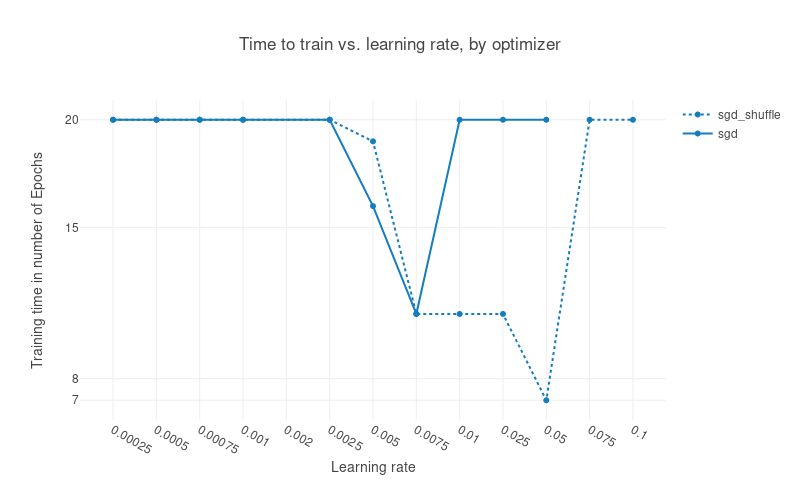
\includegraphics[scale=0.45]{images/results_sgd_shuffle} 
    \caption{Training time Stochastic Gradient Descent with input Shuffling}
    \label{fig:results_sgd}
\end{figure}
\subsection{Momentum and Nesterov}
Momentum and NAG \cite{nag} both have an additional hyperparameter $\gamma$, that, as described in Section \ref{optimizers}, defines the percentage of the previous gradient that will be added to the current gradients. We set $\gamma = 0.9$ as this is the typical value and did not alter it during our experiments. Momentum and Nesterov alone respectively only slightly decrease or increase the convergence time. Momentum optimally converges in 9 epochs and tNesterov in 13. If we combine these optimizers with input shuffling, interestingly the same phenomena as with plain SGD appear. The convergence time gets better, 8 epochs for Momentum and 3 epochs for NAG. The phenomena that a higher learning rat yields better results also happens with both of the optimizers. As Momentum does not converge in 20 epochs with a learning rate of 0.002 but does in 8 with input shuffling. 
\begin{figure}[h]
\centering
\begin{minipage}{.5\textwidth}
  \centering
      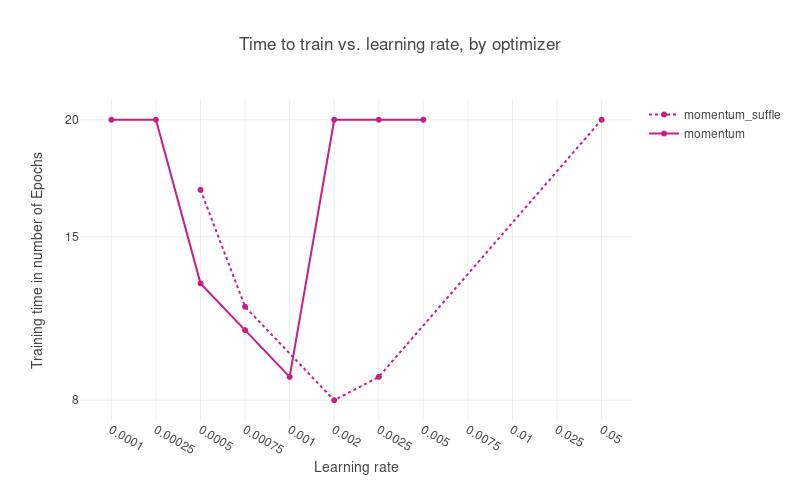
\includegraphics[scale=0.3]{images/results_mom_shuffle} 
    \caption{Training time  Momentum with input Shuffling}
    \label{fig:results_mom}
  \label{fig:test1}
\end{minipage}%
\begin{minipage}{.5\textwidth}
  \centering
    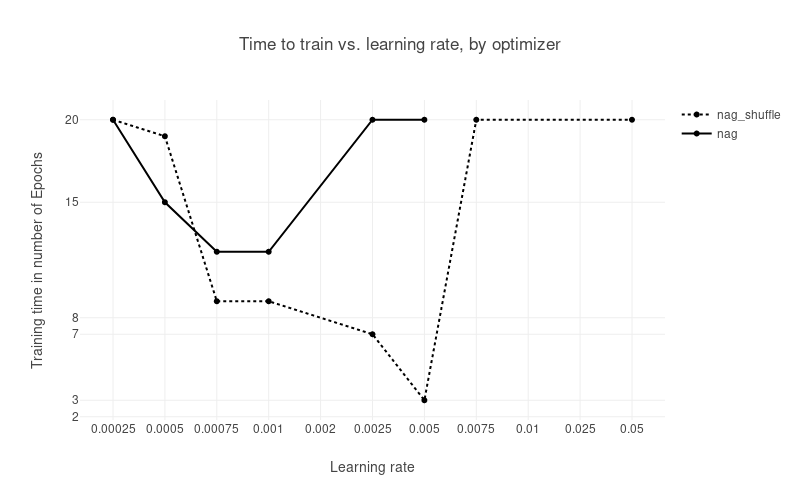
\includegraphics[scale=0.3]{images/results_nag_shuffle} 
    \caption{Training time  Nesterov with input Shuffling}
    \label{fig:results_nag}
\end{minipage}
\end{figure}
\subsection{Adagrad}
Adagrad \cite{adagrad} is a very interesting tool for learning word embeddings as it decreases the learning rate for very frequent occurring features, and vice versa (this is explained in detail in Section \ref{ssec:adagrad}). Because words that appear very frequently often do not have a semantic gain that is as important as words that appear less frequently to their context words, it's good to have a lower learning rate. So, in theory, Adagrad is particularly well suited for our task. This was confirmed empirically as our model converged in 4 epochs. When combined with shuffling adagrad only took 3 epochs to converge. This shows the tendency of the skip gram model to converge faster with input shuffling and the big impact of having different learning rate for each feature. 
Here it's interesting to notice that a higher learning rate combined with input shuffling did not yield better results than without shuffling. Both of our best results happened with a learning rate of $0.1$, as shown in Figure \ref{fig:results_adagrad_shuffle}.
\begin{figure}[h]
    \centering
            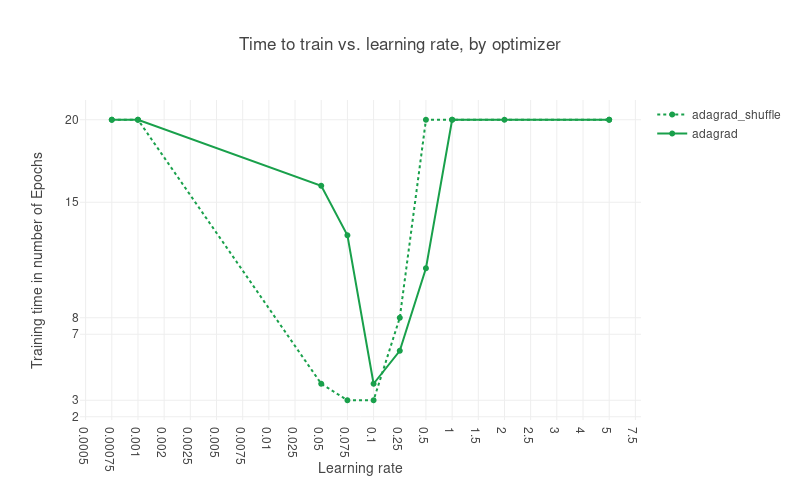
\includegraphics[scale=0.45]{images/results_adagrad_shuffle} 
    \caption{Training time Adagrad with input Shuffling}
    \label{fig:results_adagrad_shuffle}
\end{figure}
\subsection{Adadelta}
In theory Adadelta \cite{adadelta} should outperform Adagrad as it's an extension of the former. Because it didn't have any learning rate to tune, we only did 2 experiments, with and without input shuffling. We are aware of the fact that there are additional hyperparameters but did, for simplicity reason, and because their effect is not as high as the learning rate in other optimizers, decide no to tune it. We left it to its default value $\rho = 0.9$. This parameter defines the percentage taken when calculating the exponentially decaying average of past gradients, as explained in \ref{ssec:adadelta} Adadelta did not manage to achieve a word similarity of 0.66. It only converged to a similarity of 0.59. It did this in 20 epochs without input shuffling and in 3 with input shuffling, as can be seen in Table \ref{table:results_adadelta}
\begin{table}[h]
\centering
\begin{tabular}{|l|l|l|}
\hline
Adadelta Model    & Convergence Time & Word similarity \\ \hline
Without Shuffling & 20               & 0.59            \\ \hline
With Shuffling    & 3                & 0.59            \\ \hline
\end{tabular}
\caption{Convergence Time and Quality with Adadelta}
\label{table:results_adadelta}
\end{table}
\subsection{Adam}
Adam is the most advanced of all the optimizers used in our experiments and did yield the best results as seen in Figure \ref{fig:results_adam_shuffle}. Adam converged in 3 epochs without shuffling and 2 with. This is the best result that we got with any optimizer.  It's also interesting to note that as same as with Adagrad it did not react to input shuffling the same way as SGD did. In fact, it worked in the opposite direction, as we achieved our best result with input shuffling while having a lower learning rate $0.001$ then we used to achieve the best result without input shuffling $0.05$.
\begin{figure}[h]
    \centering
            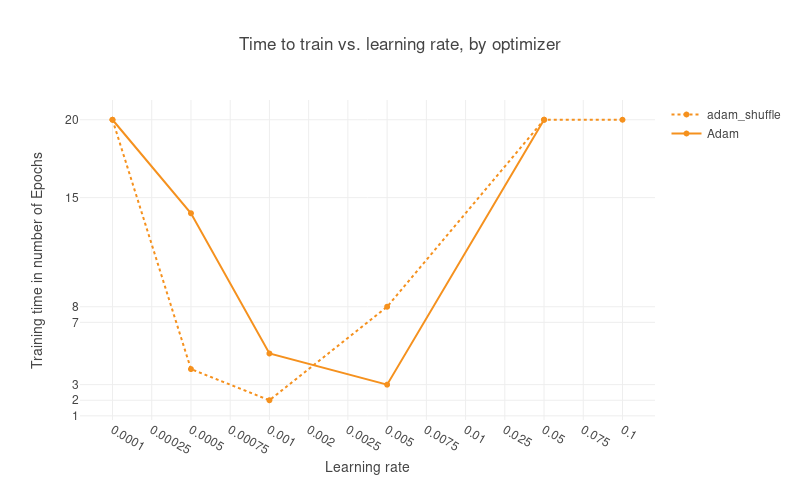
\includegraphics[scale=0.45]{images/results_adam_shuffle} 
    \caption{Training time Adam with input Shuffling}
    \label{fig:results_adam_shuffle}
\end{figure}